\documentclass[11pt,]{article}
\usepackage[left=1in,top=1in,right=1in,bottom=1in]{geometry}
\newcommand*{\authorfont}{\fontfamily{phv}\selectfont}
\usepackage[]{mathpazo}


  \usepackage[T1]{fontenc}
  \usepackage[utf8]{inputenc}



\usepackage{abstract}
\renewcommand{\abstractname}{}    % clear the title
\renewcommand{\absnamepos}{empty} % originally center

\renewenvironment{abstract}
 {{%
    \setlength{\leftmargin}{0mm}
    \setlength{\rightmargin}{\leftmargin}%
  }%
  \relax}
 {\endlist}

\makeatletter
\def\@maketitle{%
  \newpage
%  \null
%  \vskip 2em%
%  \begin{center}%
  \let \footnote \thanks
    {\fontsize{18}{20}\selectfont\raggedright  \setlength{\parindent}{0pt} \@title \par}%
}
%\fi
\makeatother




\setcounter{secnumdepth}{0}

\usepackage{color}
\usepackage{fancyvrb}
\newcommand{\VerbBar}{|}
\newcommand{\VERB}{\Verb[commandchars=\\\{\}]}
\DefineVerbatimEnvironment{Highlighting}{Verbatim}{commandchars=\\\{\}}
% Add ',fontsize=\small' for more characters per line
\usepackage{framed}
\definecolor{shadecolor}{RGB}{248,248,248}
\newenvironment{Shaded}{\begin{snugshade}}{\end{snugshade}}
\newcommand{\AlertTok}[1]{\textcolor[rgb]{0.94,0.16,0.16}{#1}}
\newcommand{\AnnotationTok}[1]{\textcolor[rgb]{0.56,0.35,0.01}{\textbf{\textit{#1}}}}
\newcommand{\AttributeTok}[1]{\textcolor[rgb]{0.77,0.63,0.00}{#1}}
\newcommand{\BaseNTok}[1]{\textcolor[rgb]{0.00,0.00,0.81}{#1}}
\newcommand{\BuiltInTok}[1]{#1}
\newcommand{\CharTok}[1]{\textcolor[rgb]{0.31,0.60,0.02}{#1}}
\newcommand{\CommentTok}[1]{\textcolor[rgb]{0.56,0.35,0.01}{\textit{#1}}}
\newcommand{\CommentVarTok}[1]{\textcolor[rgb]{0.56,0.35,0.01}{\textbf{\textit{#1}}}}
\newcommand{\ConstantTok}[1]{\textcolor[rgb]{0.00,0.00,0.00}{#1}}
\newcommand{\ControlFlowTok}[1]{\textcolor[rgb]{0.13,0.29,0.53}{\textbf{#1}}}
\newcommand{\DataTypeTok}[1]{\textcolor[rgb]{0.13,0.29,0.53}{#1}}
\newcommand{\DecValTok}[1]{\textcolor[rgb]{0.00,0.00,0.81}{#1}}
\newcommand{\DocumentationTok}[1]{\textcolor[rgb]{0.56,0.35,0.01}{\textbf{\textit{#1}}}}
\newcommand{\ErrorTok}[1]{\textcolor[rgb]{0.64,0.00,0.00}{\textbf{#1}}}
\newcommand{\ExtensionTok}[1]{#1}
\newcommand{\FloatTok}[1]{\textcolor[rgb]{0.00,0.00,0.81}{#1}}
\newcommand{\FunctionTok}[1]{\textcolor[rgb]{0.00,0.00,0.00}{#1}}
\newcommand{\ImportTok}[1]{#1}
\newcommand{\InformationTok}[1]{\textcolor[rgb]{0.56,0.35,0.01}{\textbf{\textit{#1}}}}
\newcommand{\KeywordTok}[1]{\textcolor[rgb]{0.13,0.29,0.53}{\textbf{#1}}}
\newcommand{\NormalTok}[1]{#1}
\newcommand{\OperatorTok}[1]{\textcolor[rgb]{0.81,0.36,0.00}{\textbf{#1}}}
\newcommand{\OtherTok}[1]{\textcolor[rgb]{0.56,0.35,0.01}{#1}}
\newcommand{\PreprocessorTok}[1]{\textcolor[rgb]{0.56,0.35,0.01}{\textit{#1}}}
\newcommand{\RegionMarkerTok}[1]{#1}
\newcommand{\SpecialCharTok}[1]{\textcolor[rgb]{0.00,0.00,0.00}{#1}}
\newcommand{\SpecialStringTok}[1]{\textcolor[rgb]{0.31,0.60,0.02}{#1}}
\newcommand{\StringTok}[1]{\textcolor[rgb]{0.31,0.60,0.02}{#1}}
\newcommand{\VariableTok}[1]{\textcolor[rgb]{0.00,0.00,0.00}{#1}}
\newcommand{\VerbatimStringTok}[1]{\textcolor[rgb]{0.31,0.60,0.02}{#1}}
\newcommand{\WarningTok}[1]{\textcolor[rgb]{0.56,0.35,0.01}{\textbf{\textit{#1}}}}

\usepackage{graphicx,grffile}
\makeatletter
\def\maxwidth{\ifdim\Gin@nat@width>\linewidth\linewidth\else\Gin@nat@width\fi}
\def\maxheight{\ifdim\Gin@nat@height>\textheight\textheight\else\Gin@nat@height\fi}
\makeatother
% Scale images if necessary, so that they will not overflow the page
% margins by default, and it is still possible to overwrite the defaults
% using explicit options in \includegraphics[width, height, ...]{}
\setkeys{Gin}{width=\maxwidth,height=\maxheight,keepaspectratio}

\title{NISS Data Challenge - Education, Employment, and Earnings  }



\author{\Large Nathan Nguyen\vspace{0.05in} \newline\normalsize\emph{Duke University}  }


\date{}

\usepackage{titlesec}

\titleformat*{\section}{\normalsize\bfseries}
\titleformat*{\subsection}{\normalsize\itshape}
\titleformat*{\subsubsection}{\normalsize\itshape}
\titleformat*{\paragraph}{\normalsize\itshape}
\titleformat*{\subparagraph}{\normalsize\itshape}


\usepackage{natbib}
\bibliographystyle{apsr}
\usepackage[strings]{underscore} % protect underscores in most circumstances



\newtheorem{hypothesis}{Hypothesis}
\usepackage{setspace}

\makeatletter
\@ifpackageloaded{hyperref}{}{%
\ifxetex
  \PassOptionsToPackage{hyphens}{url}\usepackage[setpagesize=false, % page size defined by xetex
              unicode=false, % unicode breaks when used with xetex
              xetex]{hyperref}
\else
  \PassOptionsToPackage{hyphens}{url}\usepackage[unicode=true]{hyperref}
\fi
}

\@ifpackageloaded{color}{
    \PassOptionsToPackage{usenames,dvipsnames}{color}
}{%
    \usepackage[usenames,dvipsnames]{color}
}
\makeatother
\hypersetup{breaklinks=true,
            bookmarks=true,
            pdfauthor={Nathan Nguyen (Duke University)},
             pdfkeywords = {pandoc, r markdown, knitr},  
            pdftitle={NISS Data Challenge - Education, Employment, and Earnings},
            colorlinks=true,
            citecolor=blue,
            urlcolor=blue,
            linkcolor=magenta,
            pdfborder={0 0 0}}
\urlstyle{same}  % don't use monospace font for urls

% set default figure placement to htbp
\makeatletter
\def\fps@figure{htbp}
\makeatother



% add tightlist ----------
\providecommand{\tightlist}{%
\setlength{\itemsep}{0pt}\setlength{\parskip}{0pt}}

\begin{document}
	
% \pagenumbering{arabic}% resets `page` counter to 1 
%
% \maketitle

{% \usefont{T1}{pnc}{m}{n}
\setlength{\parindent}{0pt}
\thispagestyle{plain}
{\fontsize{18}{20}\selectfont\raggedright 
\maketitle  % title \par  

}

{
   \vskip 13.5pt\relax \normalsize\fontsize{11}{12} 
\textbf{\authorfont Nathan Nguyen} \hskip 15pt \emph{\small Duke University}   

}

}








\begin{abstract}

    \hbox{\vrule height .2pt width 39.14pc}

    \vskip 8.5pt % \small 

\noindent This document provides an introduction to R Markdown, argues for its
benefits, and presents a sample manuscript template intended for an
academic audience. I include basic syntax to R Markdown and a minimal
working example of how the analysis itself can be conducted within R
with the \texttt{knitr} package.


\vskip 8.5pt \noindent \emph{Keywords}: pandoc, r markdown, knitr \par

    \hbox{\vrule height .2pt width 39.14pc}



\end{abstract}


\vskip 6.5pt


\noindent  \begin{Shaded}
\begin{Highlighting}[]
\CommentTok{#load data}
\NormalTok{data <-}\StringTok{ }\KeywordTok{read.csv}\NormalTok{(}\StringTok{"data/HSLSEEESAID.csv"}\NormalTok{)}
\end{Highlighting}
\end{Shaded}

\hypertarget{introduction}{%
\section{Introduction}\label{introduction}}

\begin{Shaded}
\begin{Highlighting}[]
\CommentTok{#load packages and themes}
\KeywordTok{library}\NormalTok{(showtext)}
\KeywordTok{library}\NormalTok{(tidyverse)}
\KeywordTok{font_add_google}\NormalTok{(}\StringTok{"Lora"}\NormalTok{, }\StringTok{"Lora"}\NormalTok{)}
\KeywordTok{showtext_auto}\NormalTok{()}
\end{Highlighting}
\end{Shaded}

\begin{Shaded}
\begin{Highlighting}[]
\NormalTok{order <-}\StringTok{ }\KeywordTok{c}\NormalTok{(}\StringTok{"Don't Know"}\NormalTok{, }\StringTok{"Other"}\NormalTok{, }\StringTok{"Trades and technical"}\NormalTok{, }\StringTok{"STEM"}\NormalTok{, }\StringTok{"Service"}\NormalTok{,}
            \StringTok{"Military and protective services"}\NormalTok{, }\StringTok{"Healthcare"}\NormalTok{, }\StringTok{"Education"}\NormalTok{, }
            \StringTok{"Business and Management"}\NormalTok{, }\StringTok{"Arts and entertainment"}\NormalTok{)}
\end{Highlighting}
\end{Shaded}

\begin{Shaded}
\begin{Highlighting}[]
\CommentTok{#process data }
\NormalTok{processed_data <-}\StringTok{ }\NormalTok{data }\OperatorTok
\StringTok{  }\KeywordTok{mutate}\NormalTok{(}\DataTypeTok{S4JobIndustry =} \KeywordTok{factor}\NormalTok{(S4JobIndustry, }\DataTypeTok{levels =}\NormalTok{ order)) }\OperatorTok
\StringTok{  }\KeywordTok{group_by}\NormalTok{(S4JobIndustry, X4LOCALE) }\OperatorTok
\StringTok{  }\KeywordTok{summarise}\NormalTok{(}\DataTypeTok{count_location =} \KeywordTok{n}\NormalTok{()) }\OperatorTok
\StringTok{  }\KeywordTok{group_by}\NormalTok{(S4JobIndustry) }\OperatorTok
\StringTok{  }\KeywordTok{mutate}\NormalTok{(}\DataTypeTok{count =} \KeywordTok{sum}\NormalTok{(count_location)) }\OperatorTok
\StringTok{  }\KeywordTok{mutate}\NormalTok{(}\DataTypeTok{percent =}\NormalTok{ count_location}\OperatorTok{/}\NormalTok{count}\OperatorTok{*}\DecValTok{100}\NormalTok{) }\OperatorTok
\StringTok{  }\KeywordTok{ungroup}\NormalTok{()}

\CommentTok{#create a new variable for positions of percentages on the graphs}
\NormalTok{processed_data <-}\StringTok{ }\NormalTok{processed_data }\OperatorTok
\StringTok{  }\KeywordTok{group_by}\NormalTok{(S4JobIndustry) }\OperatorTok
\StringTok{  }\KeywordTok{mutate}\NormalTok{(}\DataTypeTok{pos =} \DecValTok{100} \OperatorTok{-}\StringTok{ }\KeywordTok{cumsum}\NormalTok{(percent) }\OperatorTok{+}\StringTok{ }\NormalTok{(}\FloatTok{0.5}\OperatorTok{*}\NormalTok{percent))}
\end{Highlighting}
\end{Shaded}

\begin{Shaded}
\begin{Highlighting}[]
\KeywordTok{ggplot}\NormalTok{(processed_data, }\KeywordTok{aes}\NormalTok{(}\DataTypeTok{x =} \KeywordTok{factor}\NormalTok{(S4JobIndustry, }\DataTypeTok{levels =}\NormalTok{ order), }
                           \DataTypeTok{y =}\NormalTok{ percent,}
                           \DataTypeTok{fill =}\NormalTok{ X4LOCALE))}\OperatorTok{+}
\StringTok{  }\KeywordTok{geom_bar}\NormalTok{(}\DataTypeTok{stat =} \StringTok{"identity"}\NormalTok{, }\DataTypeTok{width =} \FloatTok{.5}\NormalTok{)}\OperatorTok{+}
\StringTok{  }\KeywordTok{coord_flip}\NormalTok{()}\OperatorTok{+}
\StringTok{  }\KeywordTok{scale_fill_manual}\NormalTok{(}\DataTypeTok{values =} \KeywordTok{c}\NormalTok{(}\StringTok{"red"}\NormalTok{, }\StringTok{"black"}\NormalTok{, }\StringTok{"blue"}\NormalTok{, }\StringTok{"grey50"}\NormalTok{))}\OperatorTok{+}
\StringTok{  }\KeywordTok{theme_linedraw}\NormalTok{()}\OperatorTok{+}
\StringTok{  }\KeywordTok{labs}\NormalTok{(}\DataTypeTok{y =} \StringTok{"Percentage"}\NormalTok{,}
       \DataTypeTok{x =} \StringTok{"Expected Job"}\NormalTok{,}
       \DataTypeTok{fill =} \StringTok{"Location"}\NormalTok{)}\OperatorTok{+}
\StringTok{  }\KeywordTok{theme}\NormalTok{(}
    \DataTypeTok{text =} \KeywordTok{element_text}\NormalTok{(}\DataTypeTok{family =} \StringTok{"Lora"}\NormalTok{, }\DataTypeTok{size =} \DecValTok{12}\NormalTok{),}
    \DataTypeTok{legend.position =} \StringTok{"bottom"}\NormalTok{,}
    \DataTypeTok{panel.grid.major.y =} \KeywordTok{element_blank}\NormalTok{(),}
    \DataTypeTok{panel.grid.minor.x =} \KeywordTok{element_blank}\NormalTok{()}
\NormalTok{  )}\OperatorTok{+}
\StringTok{  }\KeywordTok{scale_y_continuous}\NormalTok{(}\DataTypeTok{labels =} \ControlFlowTok{function}\NormalTok{(x) }\KeywordTok{paste0}\NormalTok{(x, }\StringTok{"%"}\NormalTok{))}\OperatorTok{+}
\StringTok{  }\KeywordTok{geom_text}\NormalTok{(processed_data, }\DataTypeTok{mapping =} \KeywordTok{aes}\NormalTok{(}\DataTypeTok{x =}\NormalTok{ S4JobIndustry, }
                                \DataTypeTok{y =}\NormalTok{ pos,}
                                \DataTypeTok{label =} \KeywordTok{paste0}\NormalTok{(}\KeywordTok{round}\NormalTok{(percent),}\StringTok{"%"}\NormalTok{)), }
            \DataTypeTok{size =} \DecValTok{4}\NormalTok{,}
            \DataTypeTok{color =} \StringTok{"white"}\NormalTok{)}
\end{Highlighting}
\end{Shaded}

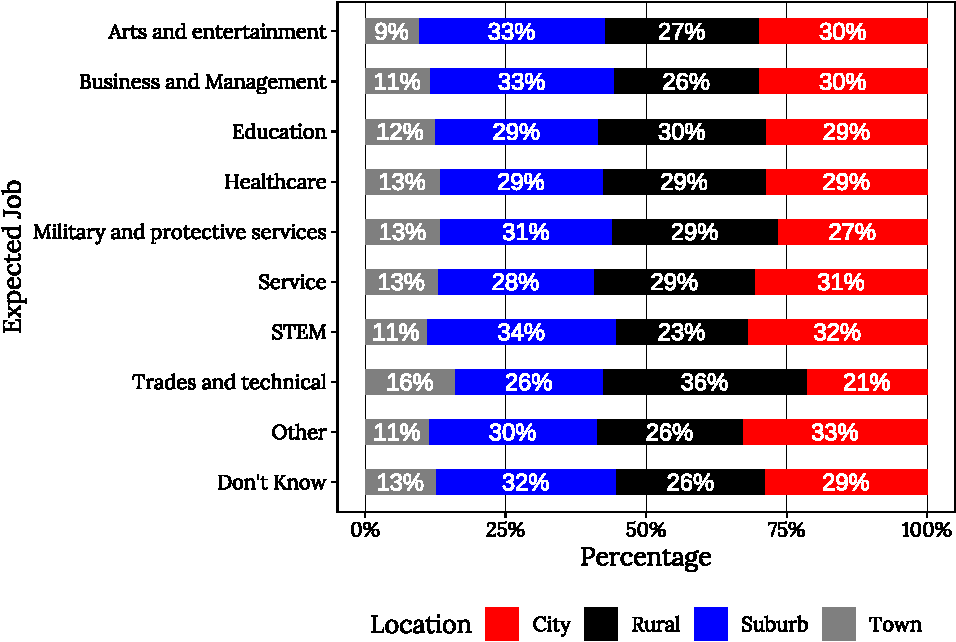
\includegraphics{Nathan-Nguyen-NISS-data-analysis_files/figure-latex/visualization-1.pdf}
\newpage
\singlespacing 
\bibliography{\textasciitilde/Dropbox/master.bib}
\end{document}